\subsection{Music recommendation}
Collaborative filtering is the part of recommender systems that predicts users' preferences for particular items. The major challenge in predicting users'listening count, as in our task, is that the available user-artist counts are usually too few and sometimes a method's performance relies on a good initial estimation of the unknown entries. 
These are reasons why we decided to implement besides the common Kmeans, KNN also ALS[cite here], which uses only the known listening counts and avoids dependency on initial estimations.

\subsection{Data description}
The training data consists in a matrix $Ytrain$ of size $1774x15082$, corresponding to $1774$ users and $15802$ artists. Element $Ytrain(i,j)$ expresses how many times user i has listened to artist j. An entry of 0 means we do not have information for that (user, artist, count) triple.
We are also given the friendship graph of the $1774$ users stored as an adjacency matrix.

\subsection{Exploratory Data Analysis}

The listening counts matrix is very sparse with a density of only $0.0026\%$, corresponding to 
$69617$ (user, artist, count) triples. 1262 artists had 0 listening counts.
The variance of the entries is very high, the highest count is $352698$ while the average listening count per user and per artist are 5.52 and 5.46 respectively.

A histogram of all the listening counts, shown in Fig\ref{fig:count_distribution} tells us that the lknown entries follow a heavy tail distribution. The long tail contains a small number of popular items, the well-known artists, and the rest are located in the heavy tail.
One method to transform skewed data such that it becomes more gaussian distributed is to use the Box-Cox transform[cite]\\
\begin{table}[h]
  \centering
  \begin{tabular}{c  c }
  $data(\lambda)$&= $log(data), \lambda = 0$ \\ 
                            &= $\frac{data^\lambda - 1}{\lambda} ,\lambda \neq 0$ \\ 
  \end{tabular}
\end{table}
. In our case, we can choose $\lambda=0$ because our values are very high and positive. This transformation will make the distances between listening counts much smaller and will reduce the influence on RMSE of the (user,artist,count) triples in the long tail. 

\begin{figure}[h]
  \centering
  \begin{subfigure}[b]{0.45\textwidth}
   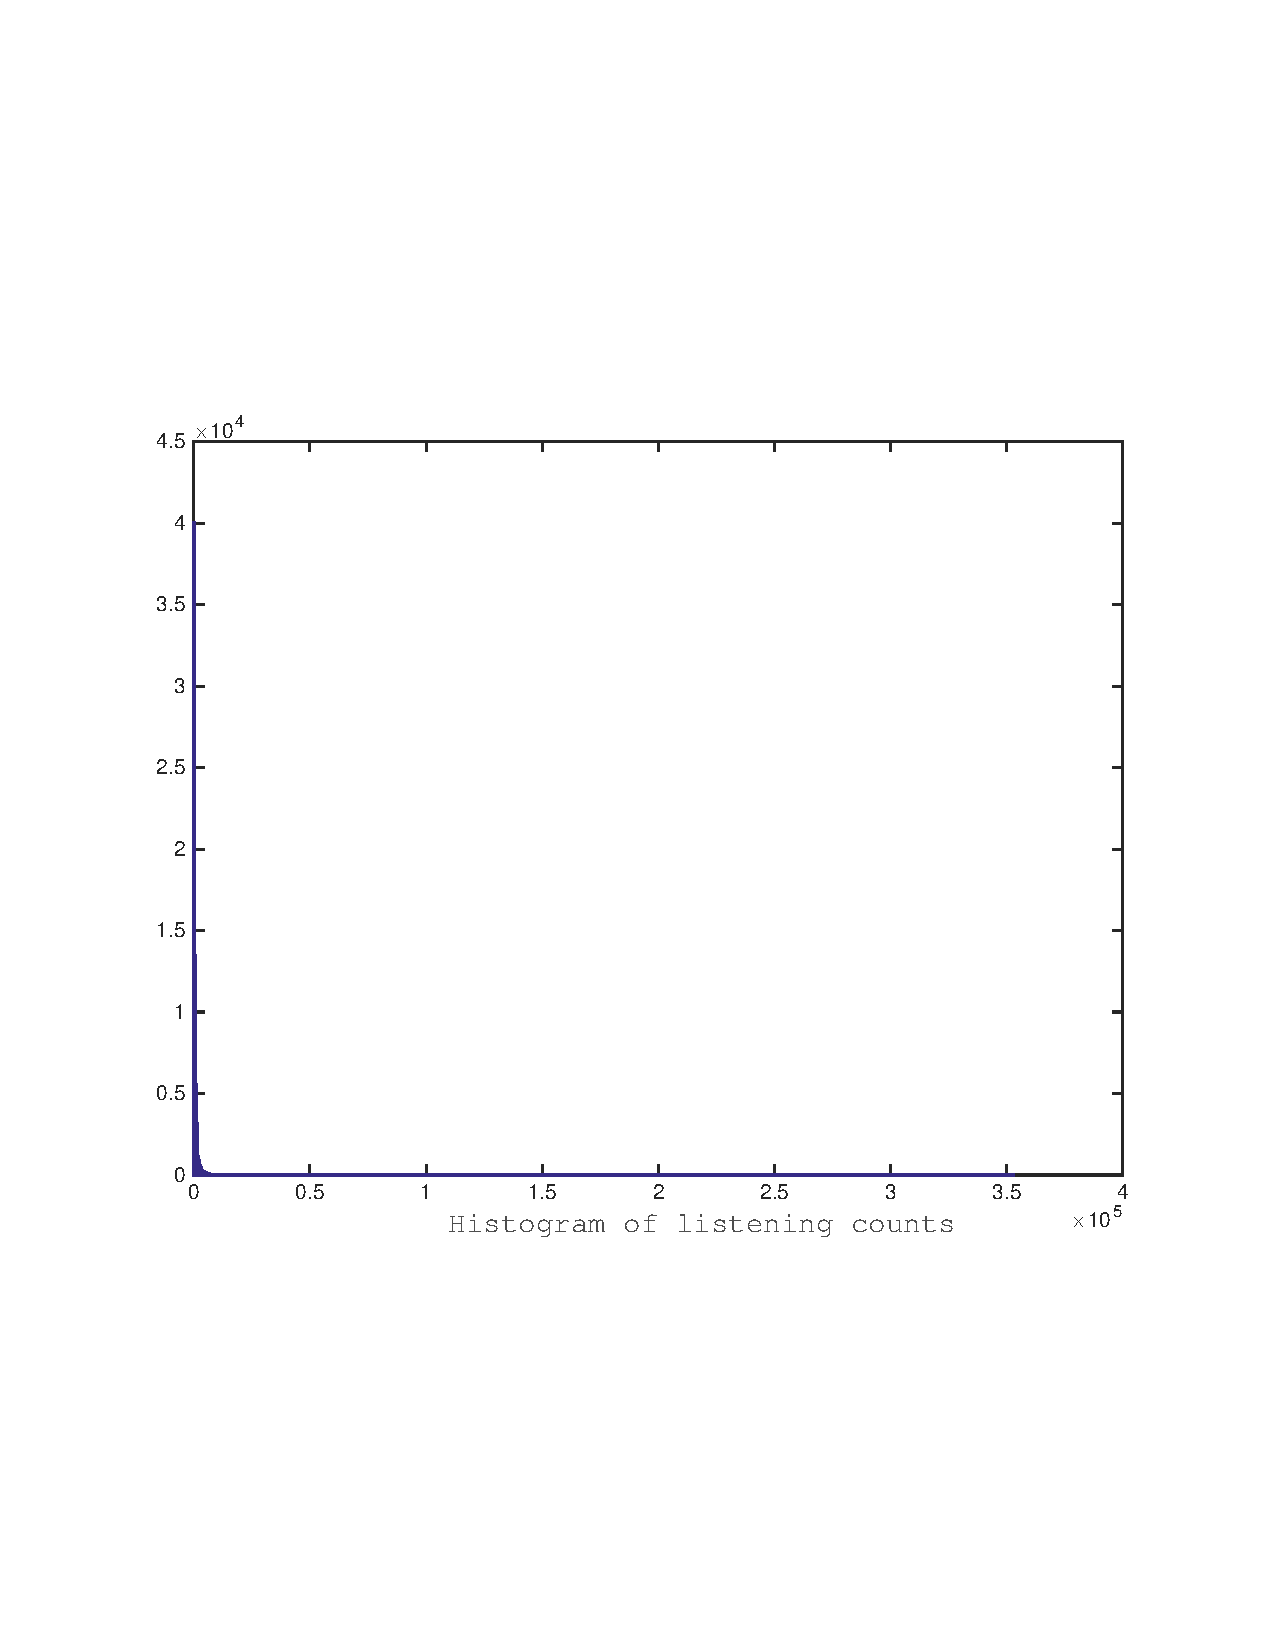
\includegraphics[width=\textwidth]{figures/histYtrain_crop.pdf}
    \caption{Before data transformation}
  \end{subfigure}
  \begin{subfigure}[b]{0.45\textwidth}
    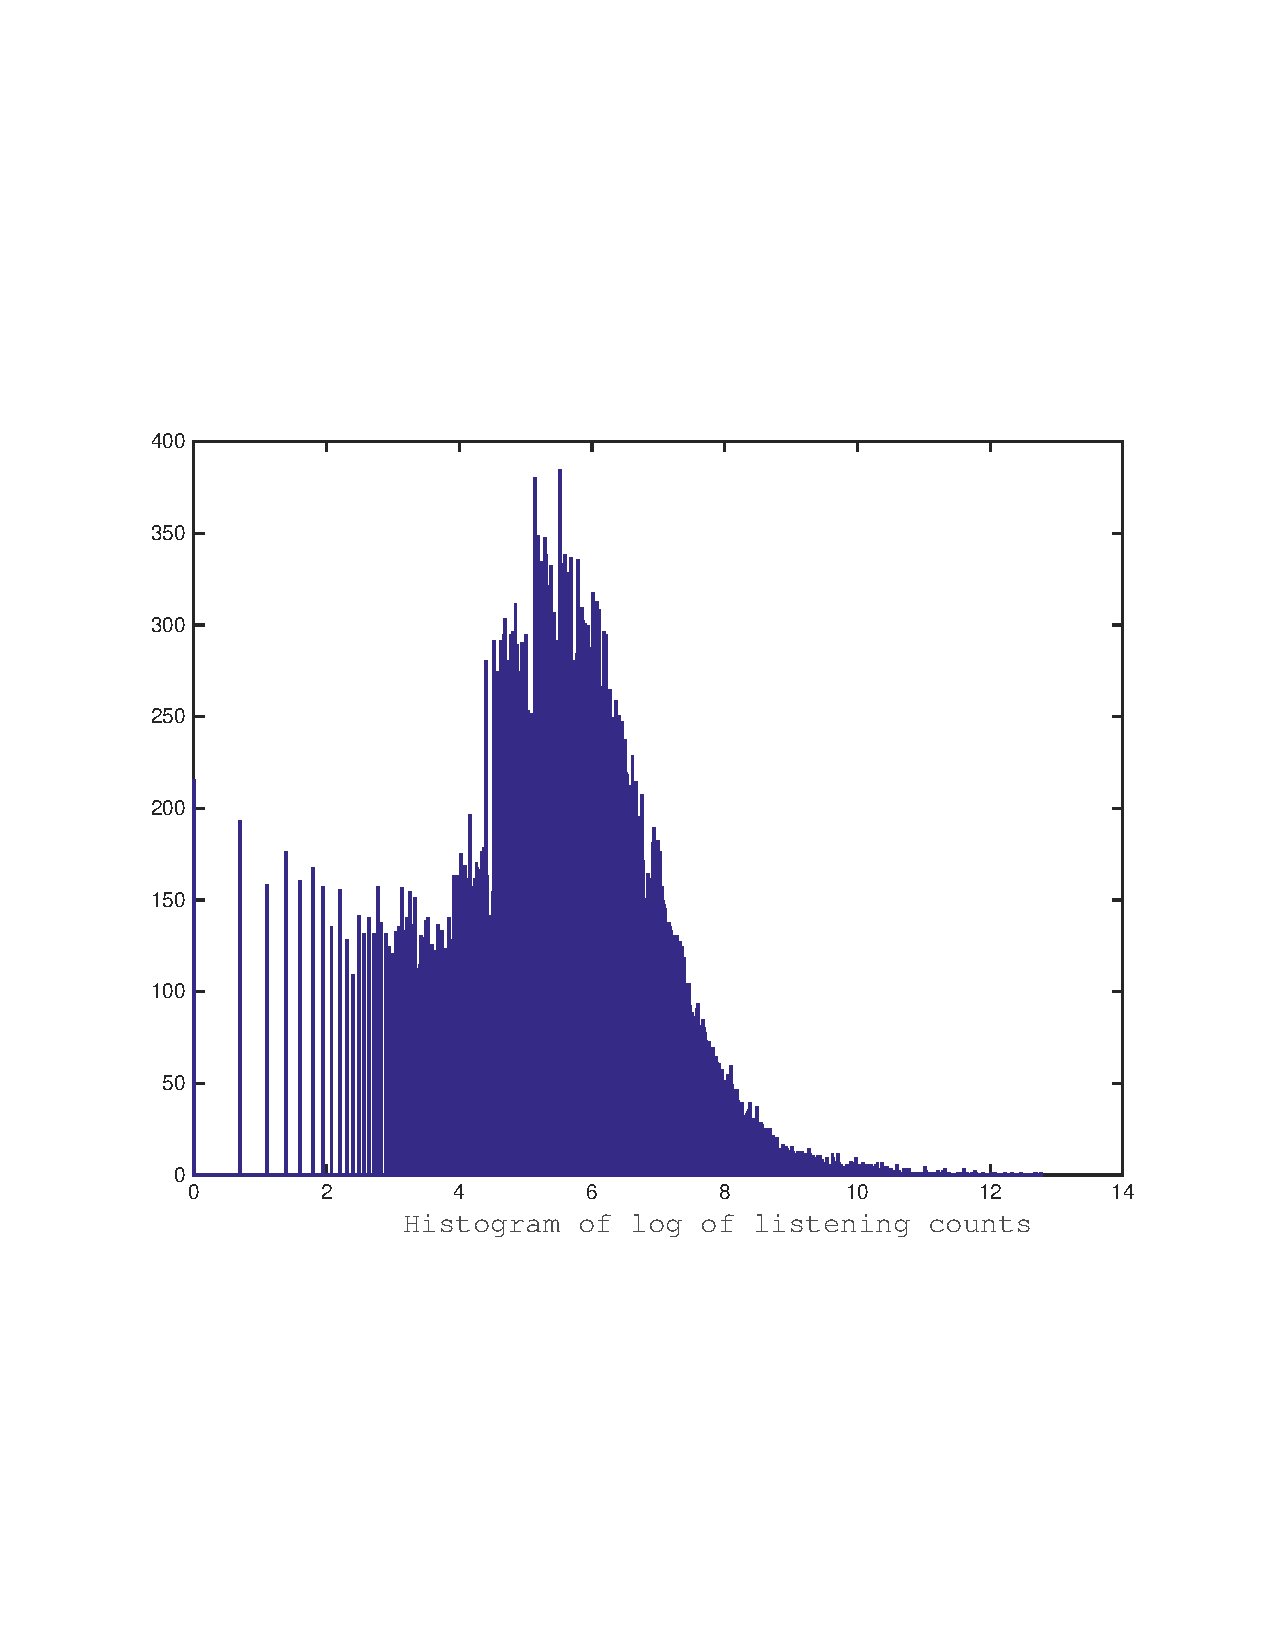
\includegraphics[width=\textwidth]{figures/histLogYtrain_crop.pdf}
    \caption{After data transformation}
  \end{subfigure}
  \caption{Distribution of all listening counts}
  \label{fig:count_distribution}
\end{figure}

\begin{figure}[h]
  \centering
  \begin{subfigure}[b]{0.45\textwidth}
   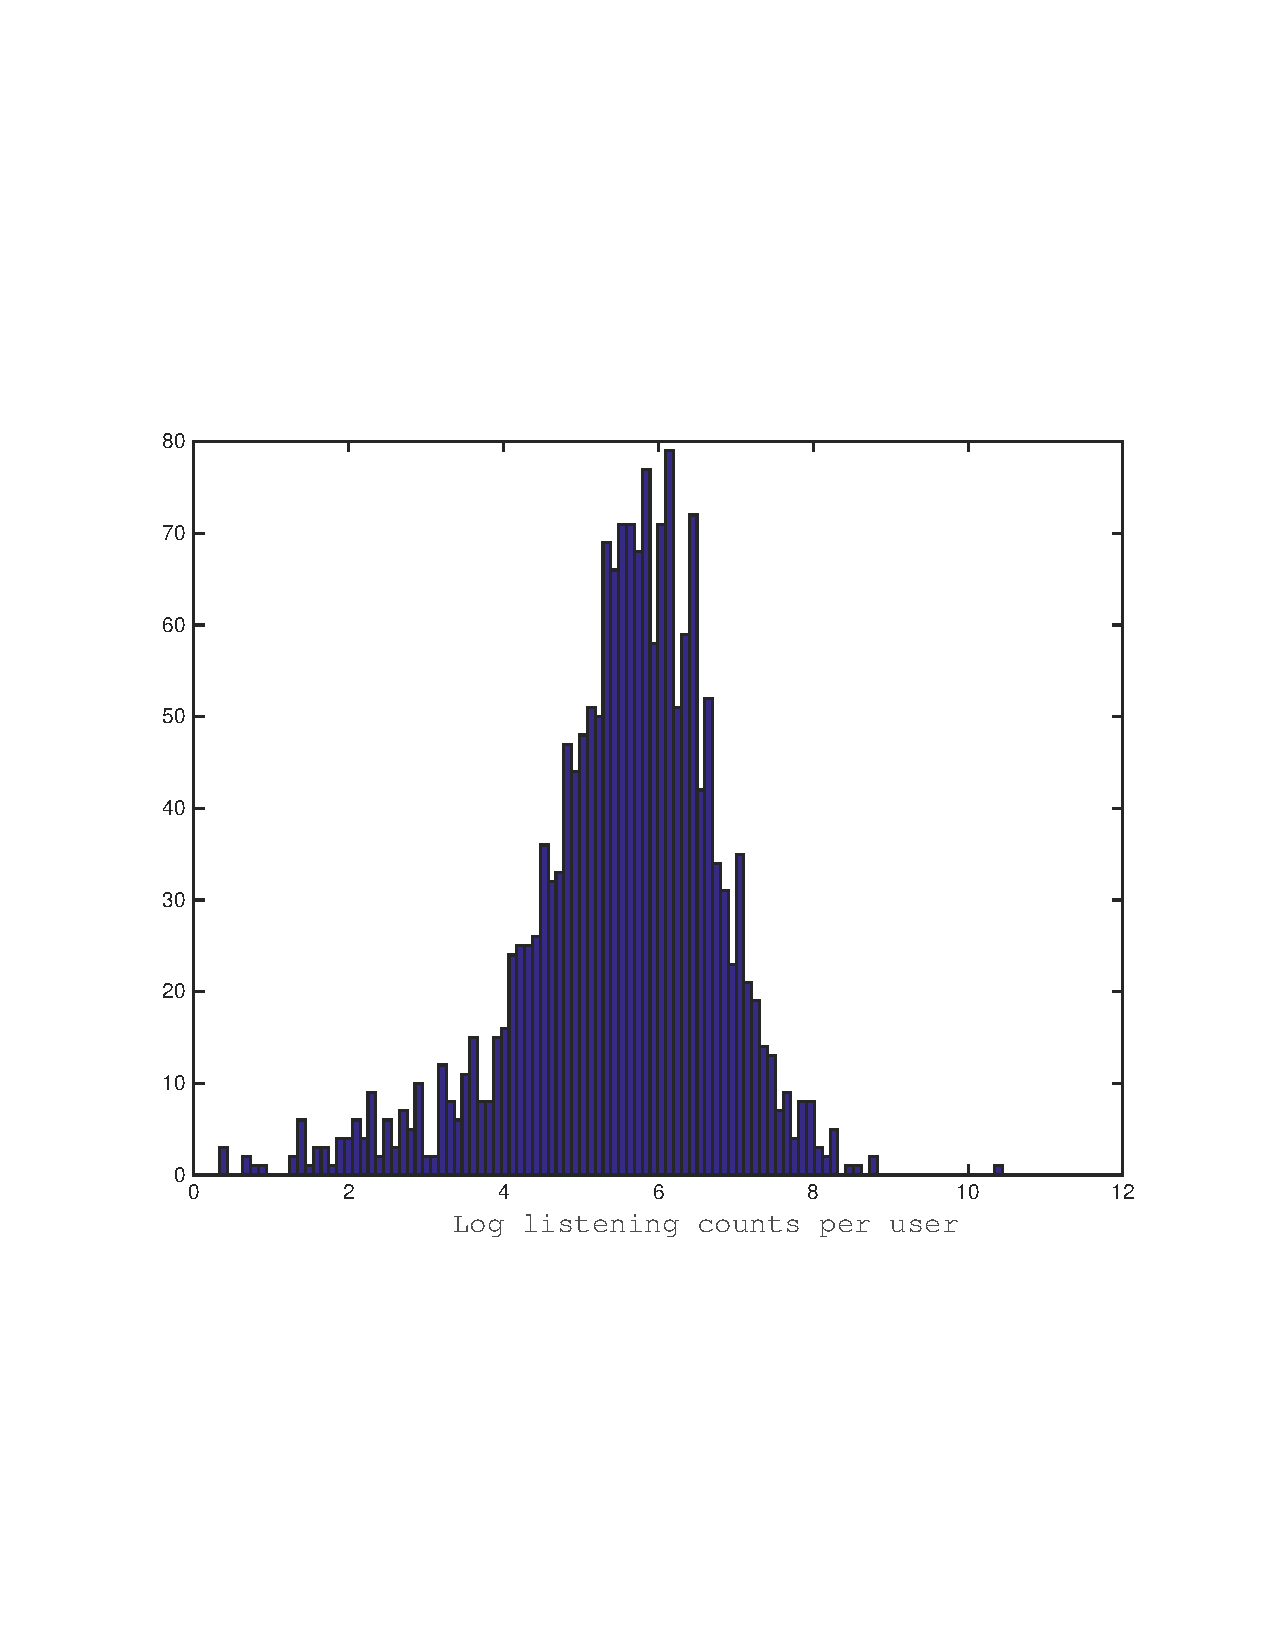
\includegraphics[width=\textwidth]{figures/histCountPerUser.pdf}
    \caption{}
  \end{subfigure}
  \begin{subfigure}[b]{0.45\textwidth}
    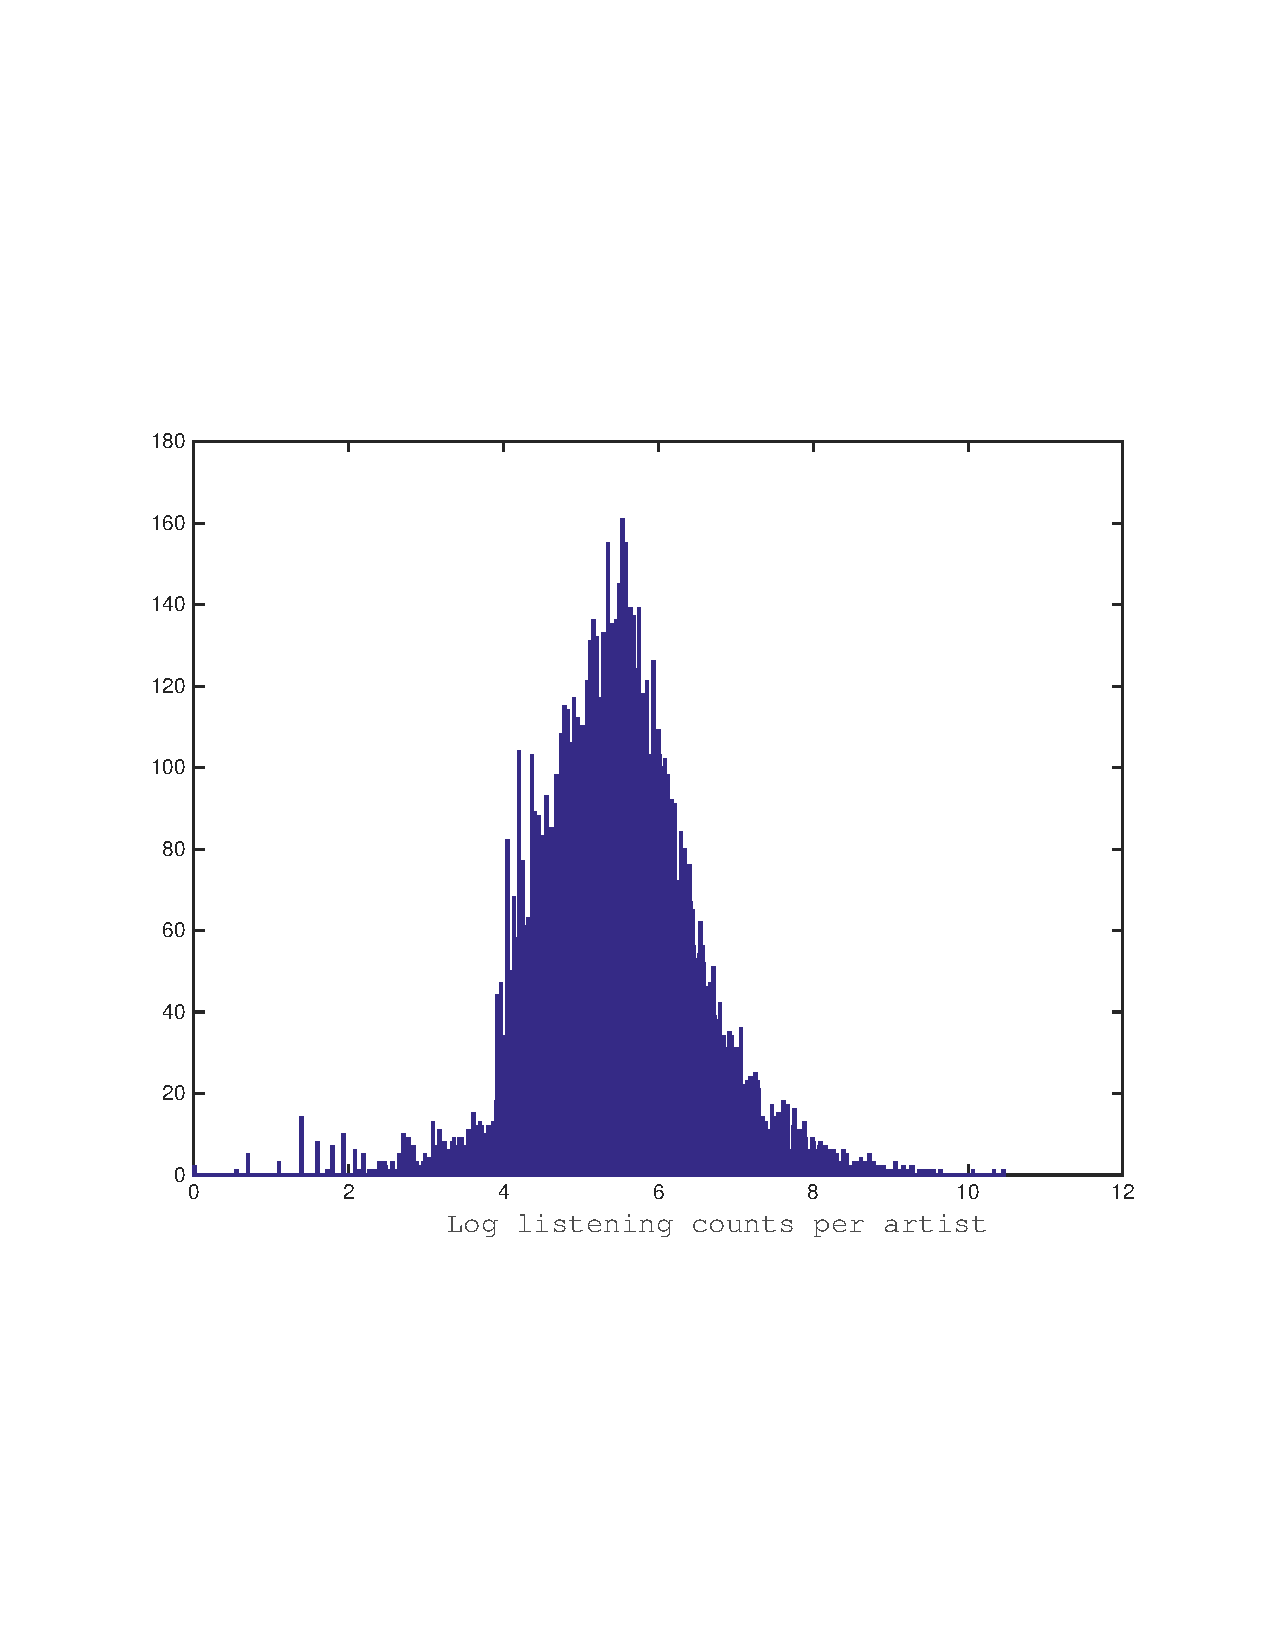
\includegraphics[width=\textwidth]{figures/histCountPerArtist.pdf}
    \caption{}
  \end{subfigure}
  \caption{Distribution per user (a) and per artist(b) log of listenining count distribution}
  \label{fig:user_artist_distribution}
\end{figure}

 
\subsection{Task 1}
In all our experiments we used 10-fold cross validation.
For the first task, we randomly omit 10 entries for every artist.
Splitting the data was more difficult since we needed to make sure we do not
remove all the entries for an artist. If an artist has $NA$ entries with $NA < 10$, then we keep $NA-1$ entries for testing,
 to still have one element for training.
We do not review here the details of ALS algorithm, the reader can consult the paper[cite] beforehand, since this was not the goal of this report.
The methods logALS and logKmeans transformed the training entries using log, but computed the RMSE undoing the transformation, by taking exp of the result.
 
\subsection{Baseline}
There are three simple basic predictions one can try: the global average count, the average count per user and the average count
per artist prediction. All of these methods give similar RMSE results: 3356, 3293 and 3496 respectively.
We note that the final RMSE is composed of various values, small and large. In Fig we can see a ploto of the RMSE error terms in log format.

\subsubsection{KNN}
\subsubsection{ALS}

\subsubsection{logALS}
Using 20 features and $lambda in [0.01,0.05,0.1,0.5,1]$ we obtain the results in table \ref{table:labda_choice} using 10-fold cross validation .The experiments were repeated twice with different seed. We note that we stopped the update steps in the algorithm only after 5 iterations because the update step was very computational intensive.
\begin{center}
  \begin{tabular}{ |l | c | c| }
    \hline
     lambda & RMSE train & RMSE test \\ \hline
     0.01   & 5075 ($\pm$  1.0793e+10) & 1.13 ($\pm$ 0.05) \\ \hline
     0.05  &  3355 ($\pm$  895)            &                1.14 ($\pm$  0.02)                   \\ \hline
     0.1     & 3350 ($\pm$ 851.5037)  & 1.58 ($\pm$ 0.0608) \\ \hline
     0.5    & 3341  ( $\pm$ 851.7858)   &13.93 ($\pm$ 0.8605)\\ \hline
     1       & 3387 ($\pm$ 842.7349)   &25.30($\pm$ 1.48)\\ \hline
     1.5    & 3416 ($\pm$ 837.1776) & 44.25($\pm$ 2.93) \\
    \hline
  \end{tabular}
  	\label{table:labda_choice}
    \captionof{table}{Estimated Train and Test RMSE for the two blob models.}
\end{center}
We can see that a value of lambda in the middle is a reaasonable choise, so we selected lambda to be 0.1 for the next experiments.
Our algorithm did a good job training  with a RMSE less than  3 but a bad job on unseen data with RMSE > 3000, meaning it is overfitting 
the training data and incrasing the value of lambda, the regularization parameter did not help.


We notice that the test error across the 10 different splits of the cross validation has values from 2000 to up to 6000. This is an artifact of the high listening counts present in the long tail and the randomness of the split.
\begin{figure}[h]
  \centering
  \begin{subfigure}[b]{0.45\textwidth}
   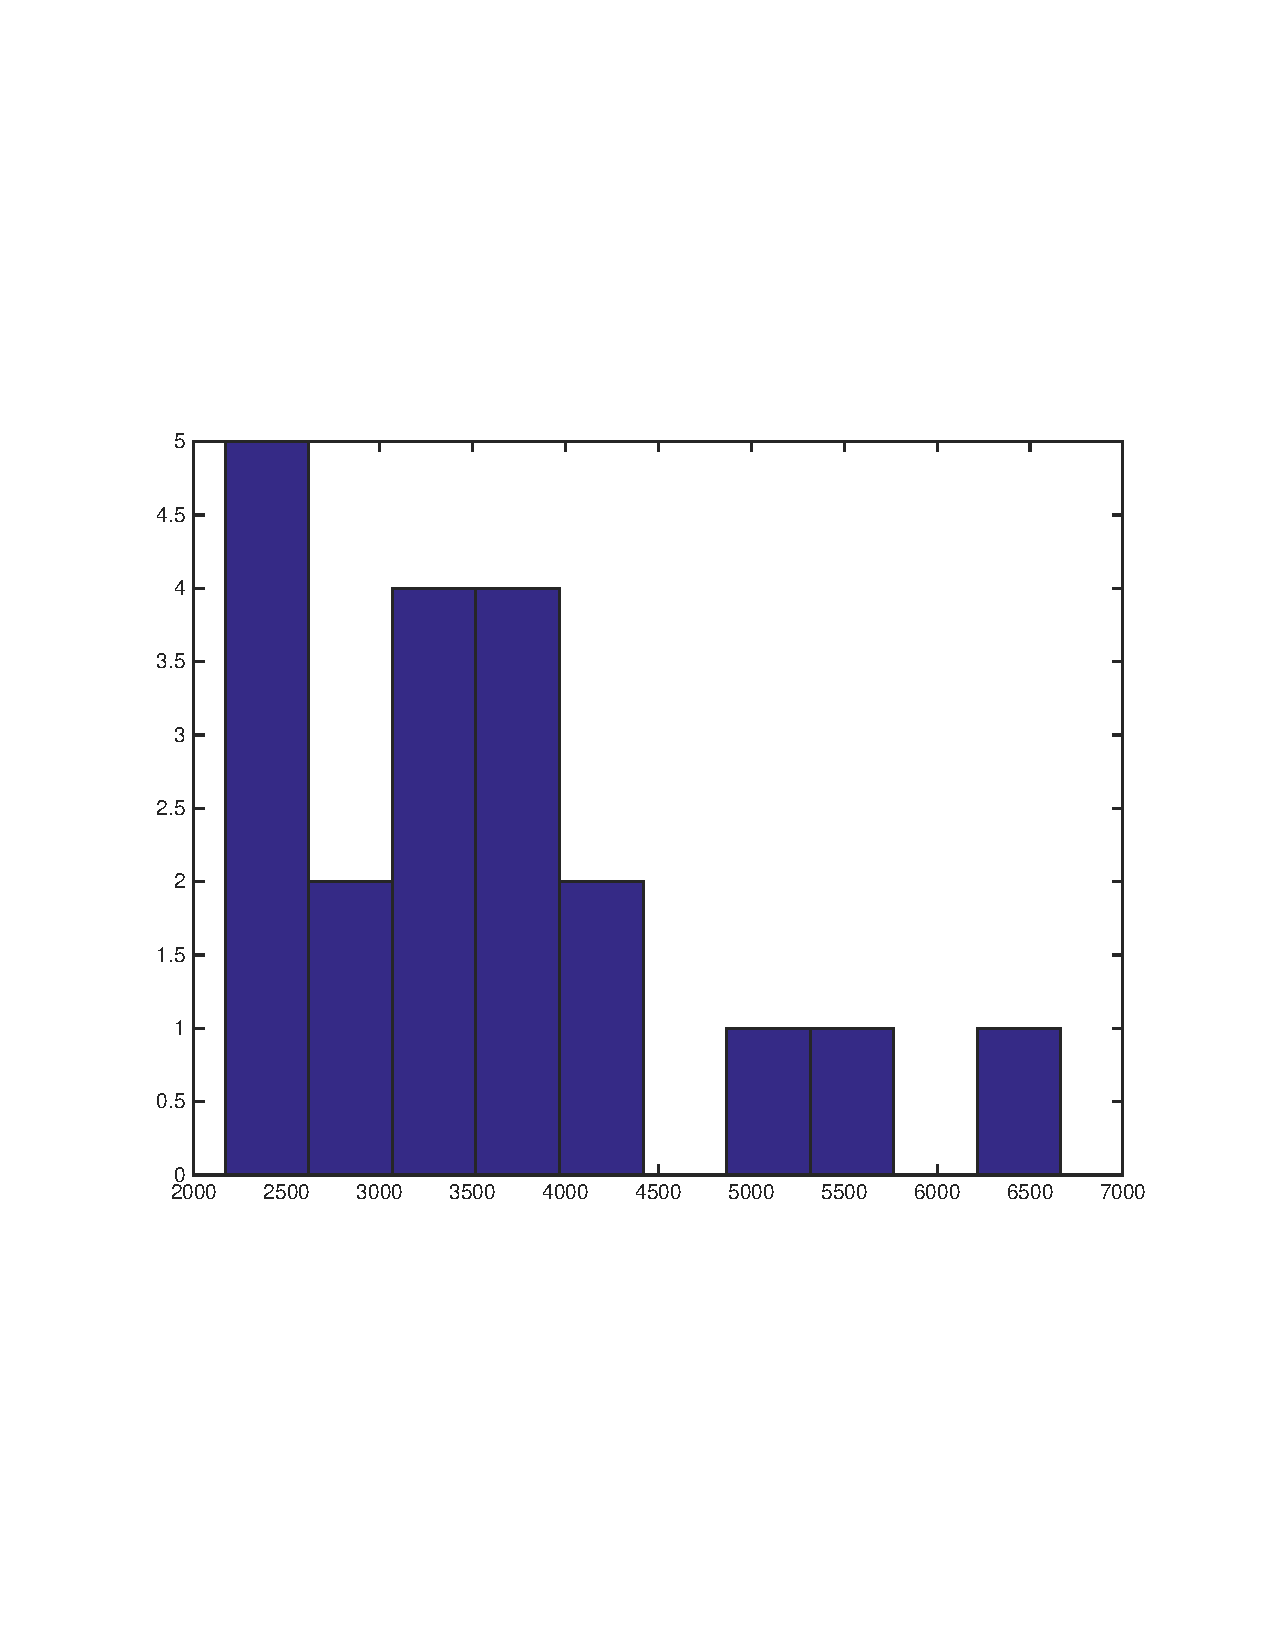
\includegraphics[width=\textwidth]{figures/distributionRMSE.pdf}
    \caption{}
  \end{subfigure}
  \begin{subfigure}[b]{0.45\textwidth}
    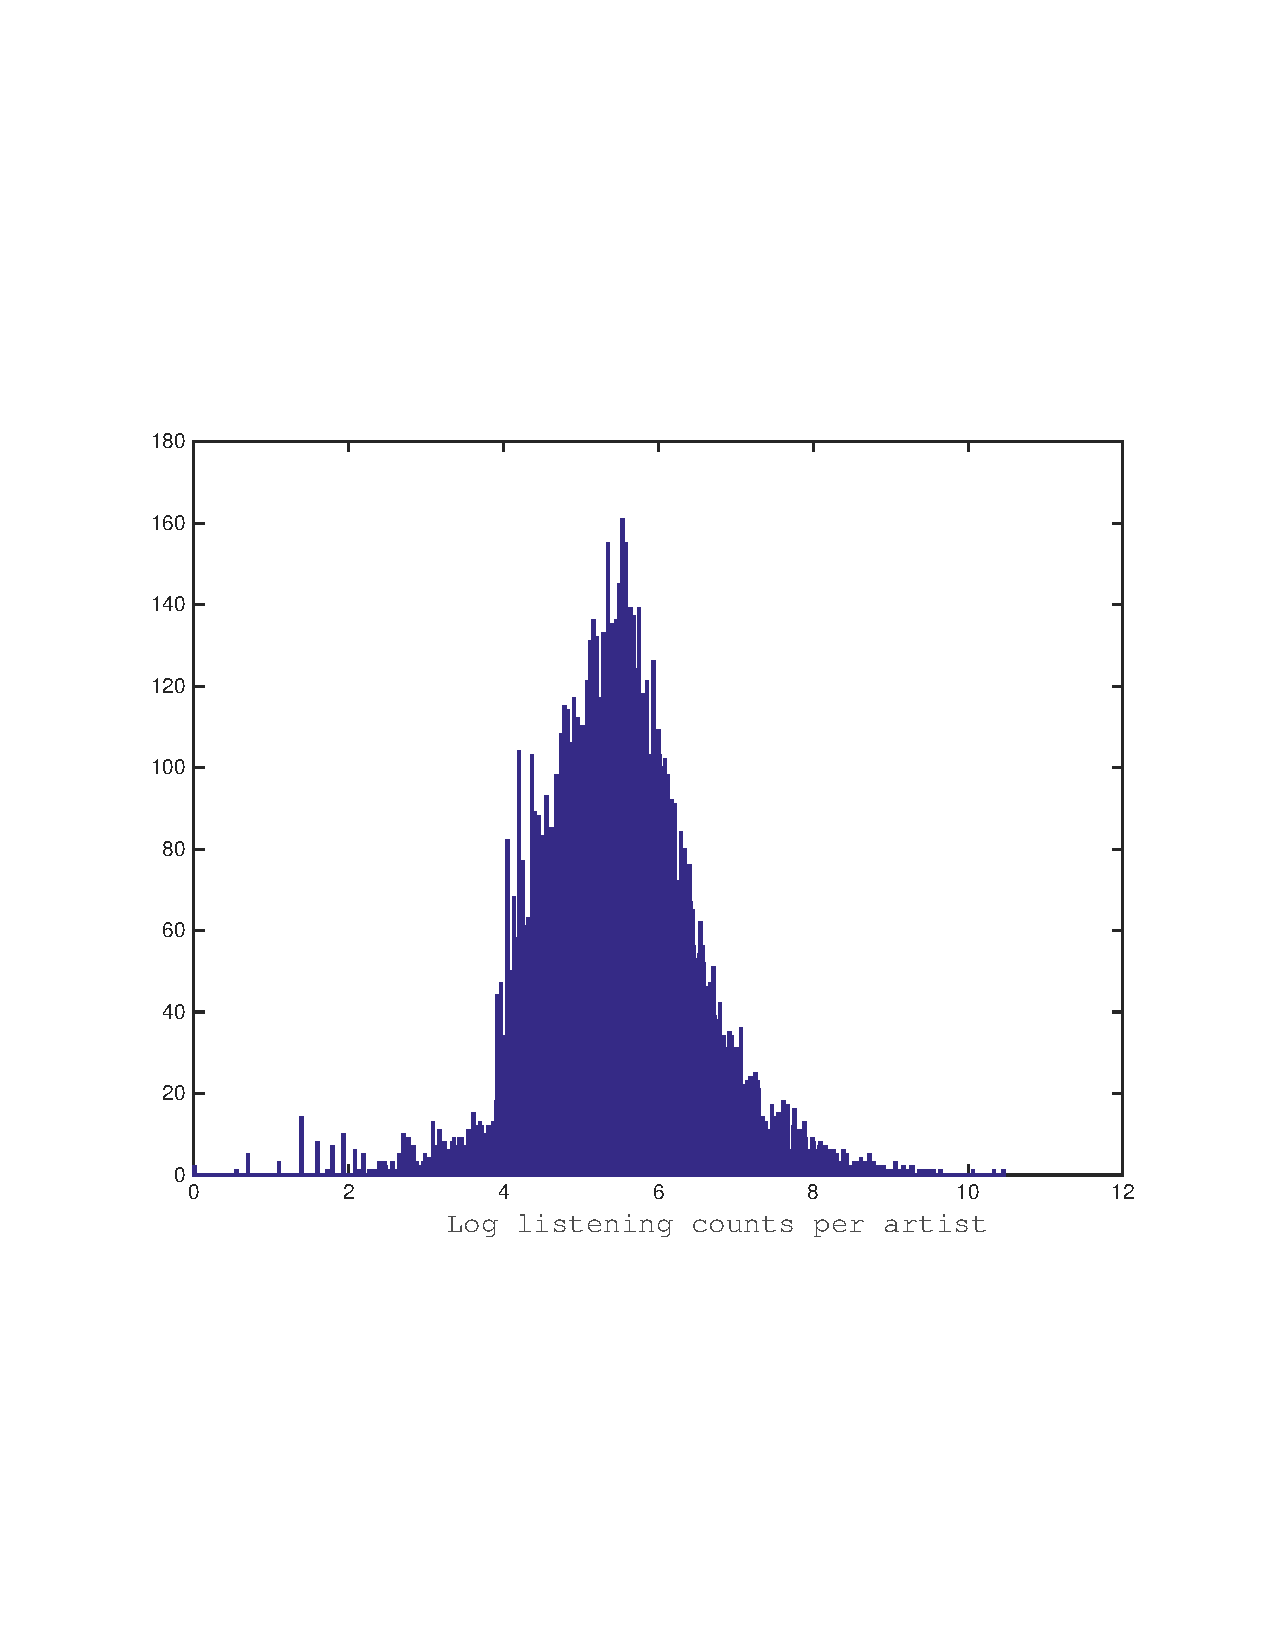
\includegraphics[width=\textwidth]{figures/histCountPerArtist.pdf}
    \caption{}
  \end{subfigure}
  \caption{Distribution per user (a) and per artist(b) log of listenining count distribution}
  \label{fig:new_plot}
\end{figure}

We varied the number of features from 10,20,30,40,50,60 with $\lambda = 0.1$. Giving train and test RMSE of 14 and 3588. So we kept the number of features to 20.
\subsubsection{Kmeans}
Inspired by the friendship graph information, we tried Kmeans with
varying values from 10 30 in steps of 5. We plot the mean train and test error using 10 fold cross validation in figure below.

We took log of the nonzeros entries of Ytrainnew and before 
computing RMSE we tranformed the data back by taking the exp
of the predicted values.
We noticed also the fact that sometimes the training error of Kmeans
(reported using exp of data) had very small fluctuations and it was not always decreasig as the algorithm convergence properties would expect. This is due to the fact that Kmeans miminizes squared error but our cost is a little different since we transform the data using exp.

We had avary large variations in the algorithm's output.

One reason for performing Kmeans for clusteringover users 
instead of over artists, although the number of artists is larger than the number of users is to be easier in Task 2.



We can see that our algorithm performs for

\subsection{Task 2}
\subsubsection{Friendship information}
Regarding the friendshiop information, we noticed there are 22 connected components, but many of them contained.
1776 nodes and 22904 edges.
Using Vincent D Blondel, Jean-Loup Guillaume, Renaud Lambiotte, Etienne Lefebvre, Fast unfolding of communities in large networks, in Journal of Statistical Mechanics: Theory and Experiment 2008 (10), P1000 and the Gephi tool to find properties of the graph, it suggested it has about
32 communities, of which 8 had more than 150 members and the others being very small. (22 connected components, of which 20 are very small < 50 users.) This was run to give us an idea of the number of clusters we could use in Kmeans.

\subsection{•}
In this task we are given a set of new users and their friendship information.
The task is to predict their listening counts based only on their friendship information with
people for which we already have some information about their listening habbits.
We experiment with three methods.
 A baseline method in which a (user,artist) count is predicted
using the average count of its friends, global average if that informatino id not present.

The second method uses the 20 clusters from the previous method and predicts the count
as an average weight of the listening counts of the clusters of the friends.

The thirs method uses the 20 clusters from the previous method in a weighted average approach but this time also the friends of the friends information is used. 

\subsection{Summary}



